\chapter{Musik}
I dette afsnit vil der blive analyseret 5 forskellige musiksekvenser, vi selv har valgt. \\
Der vil være 4 forskellige grafer for hver musiksekvens.\\ \\
Den første viser signalet som funktion af tiden - her befinder signalet sig i tidsdomænet. \\
De 2 næste viser signalet magnitude som funktion af frekvens i Hz. Den sidste af disse viser signalet på en logaritmisk x-akse. \\
Den sidste graf viser fasen som funktion af frekvens i Hz. De sidste 3 befinder sig frekvens-domænet, da vi har lavet en DFT af signalet.   

\section{Cool music}

\begin{figure}[H]
	\centering
	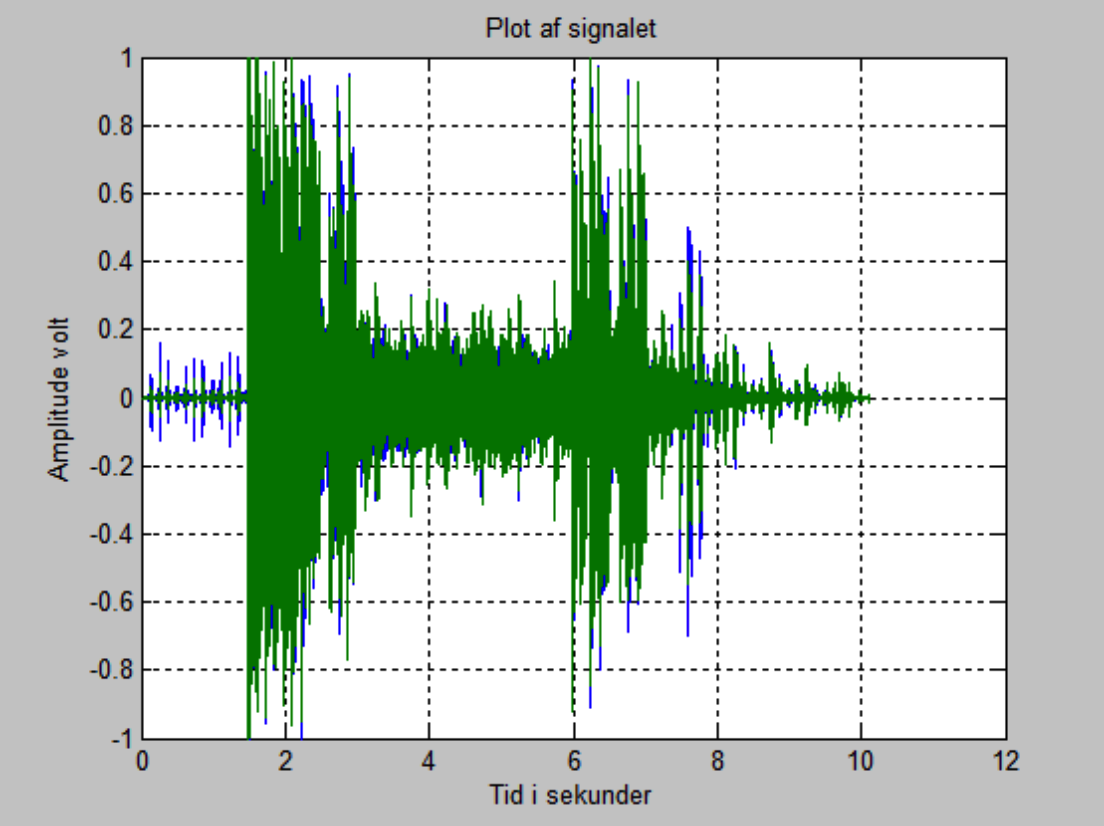
\includegraphics[width=0.7\textwidth]{Figurer/Snip20151001_3}
	\caption{\textit{Cool music} - Signalet amplitude som funktion af tiden i sekunder}
\end{figure}

Det er et stykke elektronisk musik på 10 sekunder. Vi kan se, at der er nogle store amplituder flere steder i musiksekvensen. I det første område med store amplituder, er der en tromme, der går lidt mere amok i forhold til resten af sekvensen. Den sidste halvdel med store amplituder bliver der scratchet og så dør sekvensen ud.

\begin{figure}[H]
	\centering
	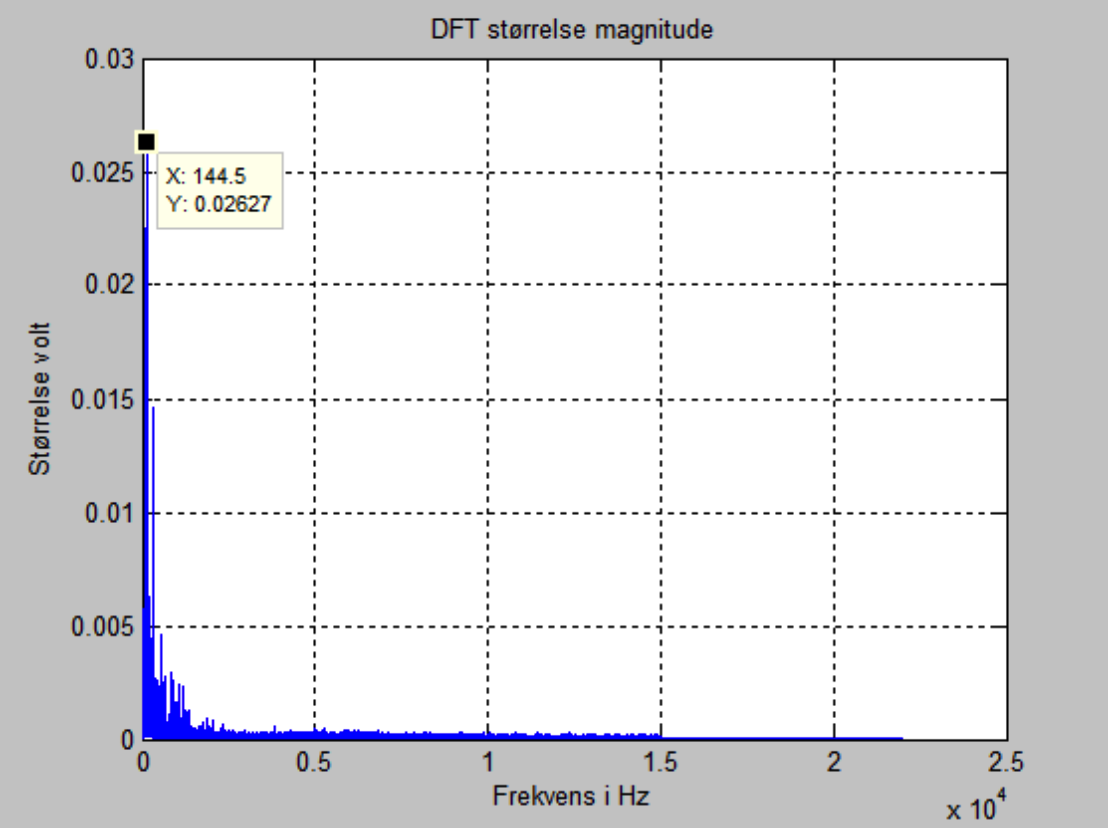
\includegraphics[width=0.7\textwidth]{Figurer/Snip20151001_7}
	\caption{\textit{Cool music} - Signalets magnitude som funktion af frekvens i Hz}
\end{figure}

Fra 0 til 500 Hz er der meget energi i musiksekvensen - dette kan vi se, da der er en meget høj volt (ca. 0,005-0,025) i dette område i forhold til resten af sekvensen, som ligger imellem 0-0,005. Den største amplitude ligger ved 144,5 Hz.      

\begin{figure}[H]
	\centering
	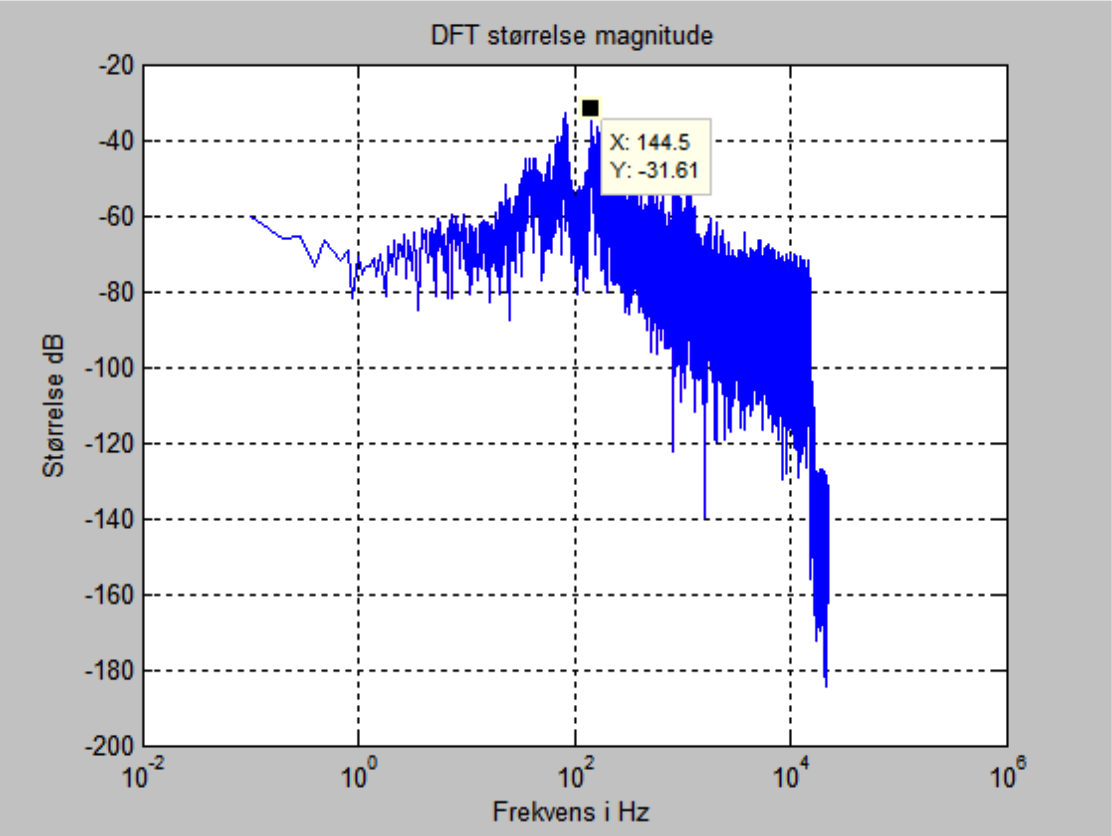
\includegraphics[width=0.7\textwidth]{Figurer/Snip20151001_8}
	\caption{\textit{Cool music} - Signalets magnitude som funktion af frekvens i Hz. Logaritmisk x-akse}
\end{figure}  

Vi har valgt, at plotte musiksekvensen med en logaritmisk x-aksen, da det på den måde bliver mere tydeligt, hvordan signalet opfører sig. Y-aksen bliver et udtryk af størrelse målt i dB. \\
Vi kan se, at den største amplitude også her ligger ved 144,5 Hz. Denne frekvens ligger tæt på D3 tonen, som er på 146,832 Hz.      


\begin{figure}[H]
	\centering
	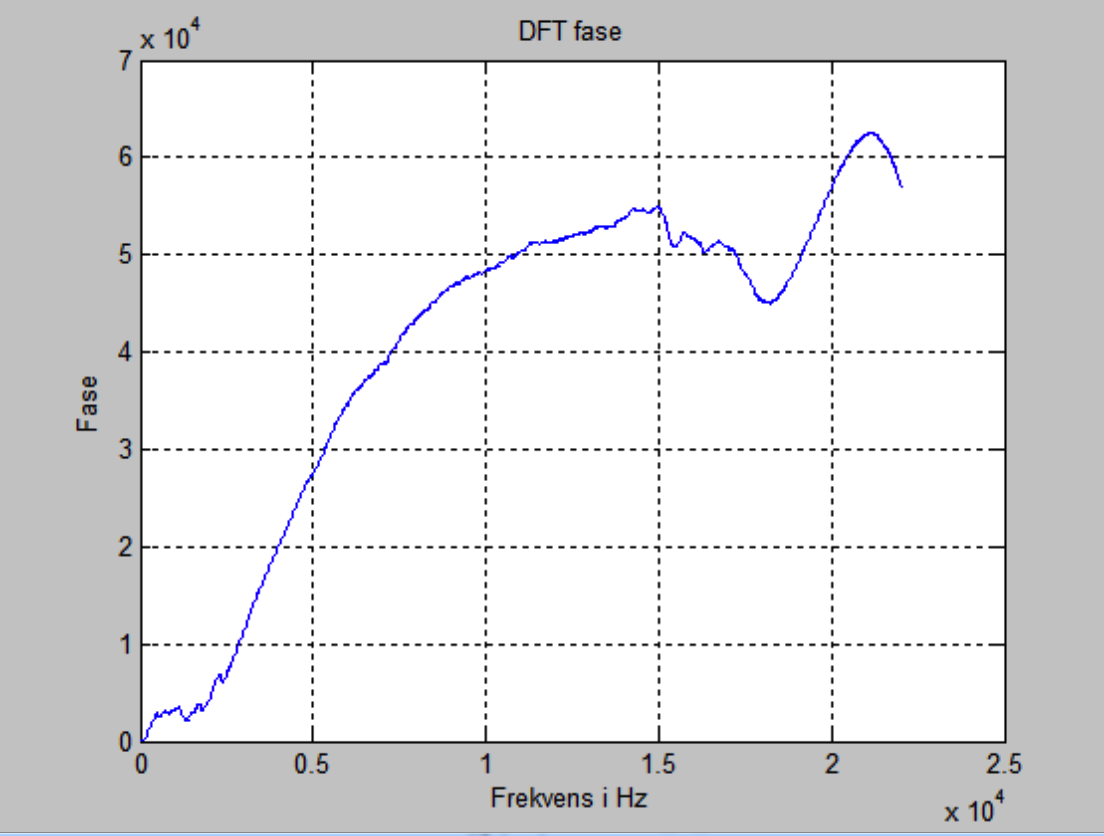
\includegraphics[width=0.7\textwidth]{Figurer/Snip20151001_6}
	\caption{\textit{Cool music} - Signalets fase som funktion af frekvens i Hz}
\end{figure} 

Der er fasedrejninger fra 15000 Hz til 22000 Hz. 

\section{Drum roll}
 
\begin{figure}[H]
	\centering
	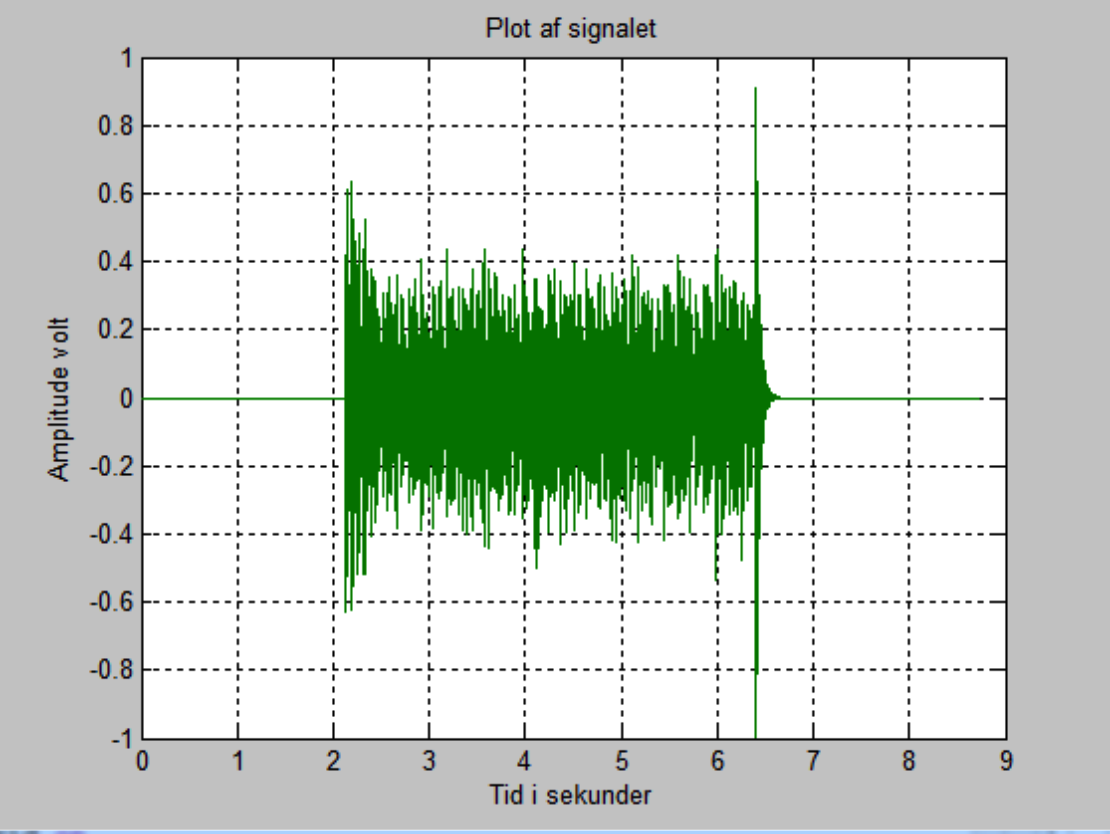
\includegraphics[width=0.7\textwidth]{Figurer/Snip20151001_9}
	\caption{\textit{Drum roll} - Signalet amplitude som funktion af tiden i sekunder}
\end{figure}

Hvis man ser bort fra 2,5 sekund og de sidste 3 sekunder, ses det at amplitudespekteret ikke varier ret meget, hvilket vil sige, at det er meget monotont. Det stemmer meget overens med, når man lytter til musiksekvensen. Der er 2 pauser i sekvensen - i starten og tilsidst. Det kan vi se ved, at der ingen amplitude er - den ligger bare konstant på 0. Lige når trommens lyd begynder er der en større aktivitet end i det monotone afsnit. Ved 6,3 sekunder befinder den største amplitude sig - her bliver der i musiksekvensen muligvis slået ekstra meget i trommen.  

\begin{figure}[H]
	\centering
	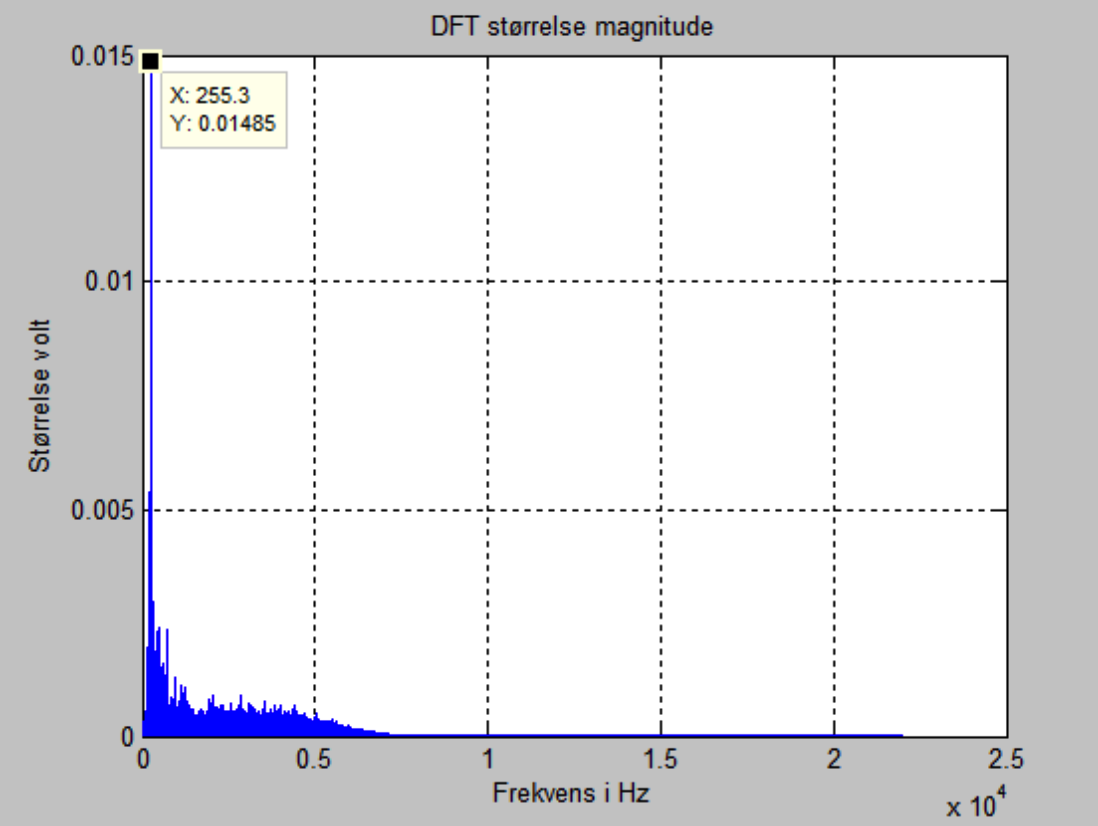
\includegraphics[width=0.7\textwidth]{Figurer/Snip20151001_14}
	\caption{\textit{Drum roll} - Signalets magnitude som funktion af frekvens i Hz}
\end{figure}

 Den største amplitude ligger ved 255,3 Hz. Frekvenserne efter ca. 500 Hz har en markant lavere energi.

\begin{figure}[H]
	\centering
	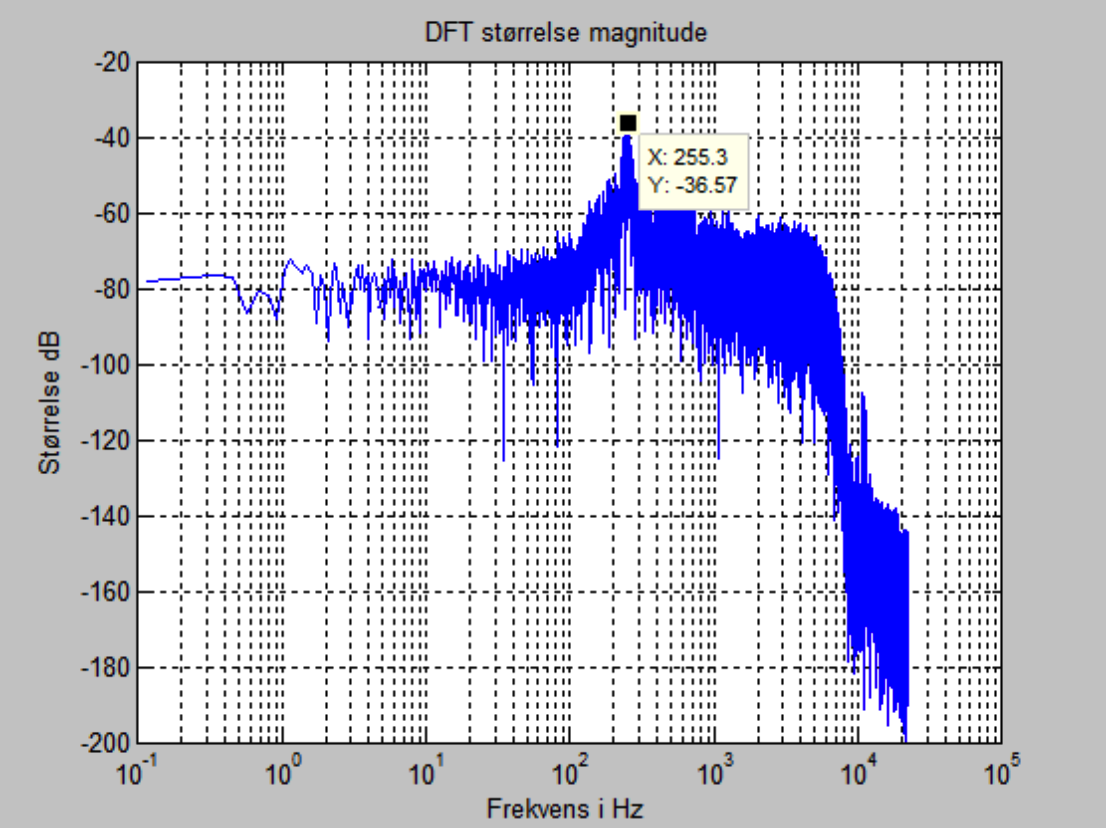
\includegraphics[width=0.7\textwidth]{Figurer/Snip20151001_12}
	\caption{\textit{Drum roll} - Signalets magnitude som funktion af frekvens i Hz. Logaritmisk x-akse}
\end{figure} 

Vi har valgt, at plotte musiksekvensen med en logaritmisk x-aksen, da det på den måde bliver mere tydeligt, hvordan signalet opfører sig. Y-aksen bliver et udtryk af størrelse målt i dB. \\
Vi kan se, at den største amplitude også her ligger ved 255,3 Hz. Denne frekvens ligger forholdsvis tæt på C4 tonen, som er på 262 Hz.   

\begin{figure}[H]
	\centering
	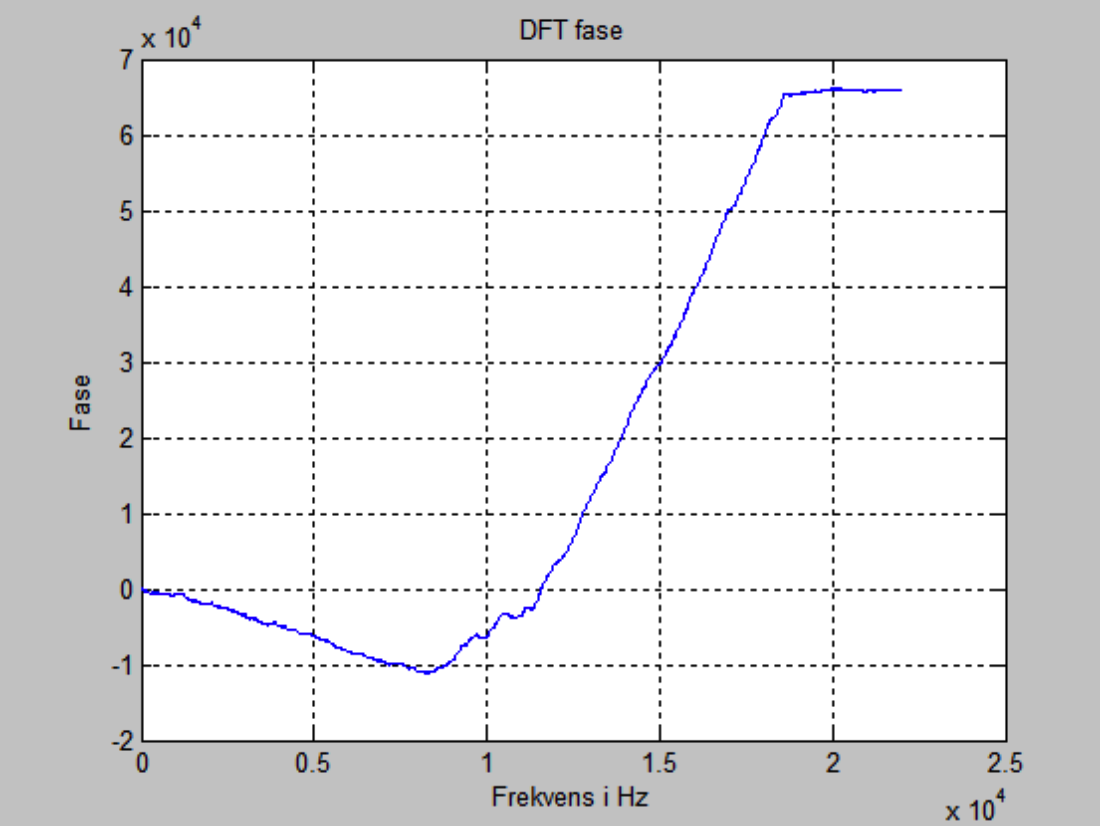
\includegraphics[width=0.7\textwidth]{Figurer/Snip20151001_15}
	\caption{\textit{Drum roll} - Signalets fase som funktion af frekvens i Hz}
\end{figure} 

Der ses en fasedrejning ved ca. 8000 Hz, hvorefter fasen stiger kontinuerligt til ca. 18000 Hz.

\section{Straight outta Compton}

\begin{figure}[H]
	\centering
	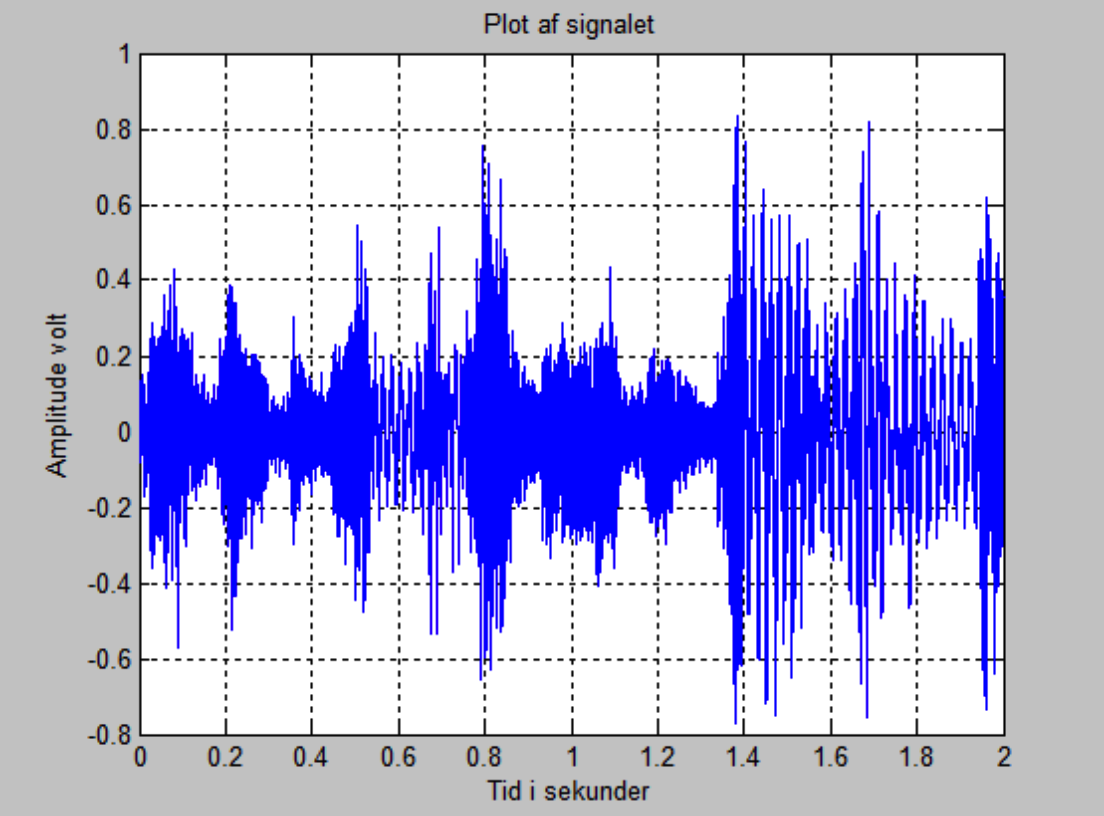
\includegraphics[width=0.7\textwidth]{Figurer/Snip20151001_16}
	\caption{\textit{Straight outta Compton} - Signalet amplitude som funktion af tiden i sekunder}
\end{figure}

Vi arbejder her med gruppen N.W.A. og deres nummer 'Straight outta Compton', hvor vi har valgt, at kigge nærmere på en lydsekvens fra 92 sekunder inde i sangen. Den lydsekvens vi har kigget på strækker sig over 2 sekunder. Lige som med 'Uptown funk' i musikstykke 4, så ses det, at denne lydsekvens ligeledes benytter et bredt amplitudespekter. Specielt fra 1,35 sekunder stiger amplituden markant, hvorefter den svinger voldsomt resten af lydsekvensen.

\begin{figure}[H]
	\centering
	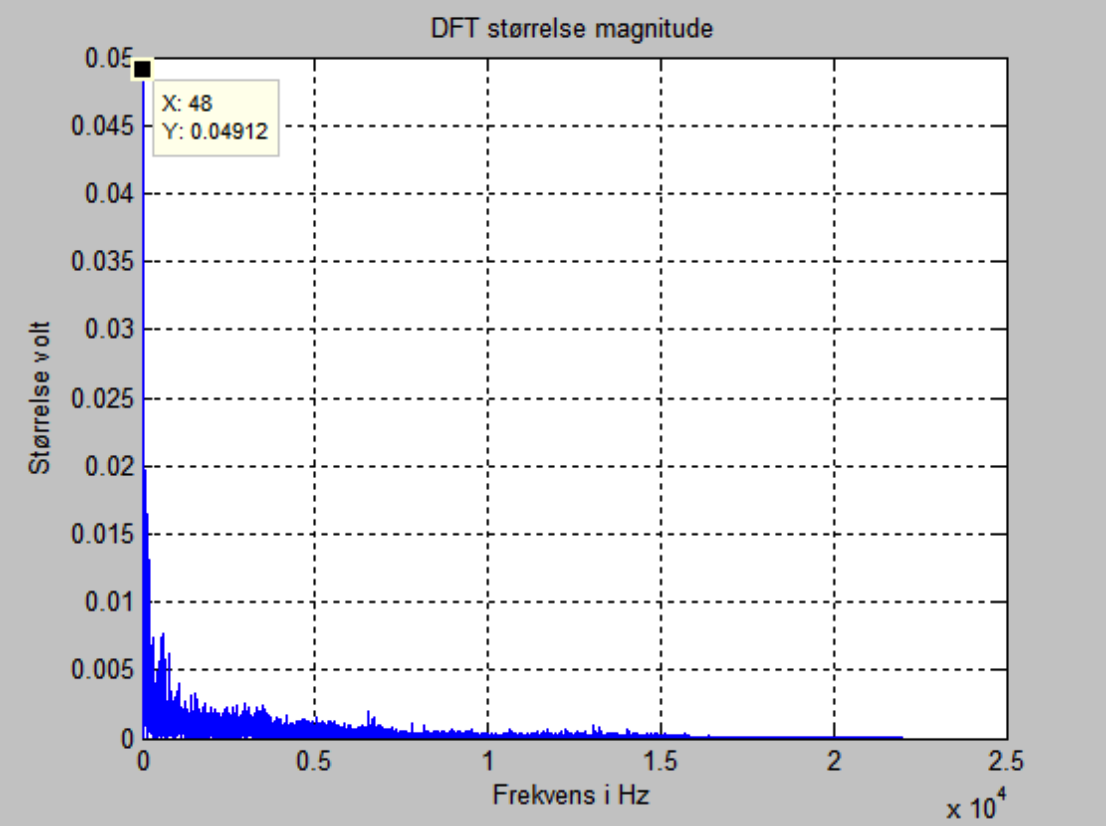
\includegraphics[width=0.7\textwidth]{Figurer/Snip20151001_17}
	\caption{\textit{Straight outta Compton} - Signalets magnitude som funktion af frekvens i Hz}
\end{figure}

Den største amplitude liger ved 48 Hz. Frekvenserne derefter har en markant lavere energi.

\begin{figure}[H]
	\centering
	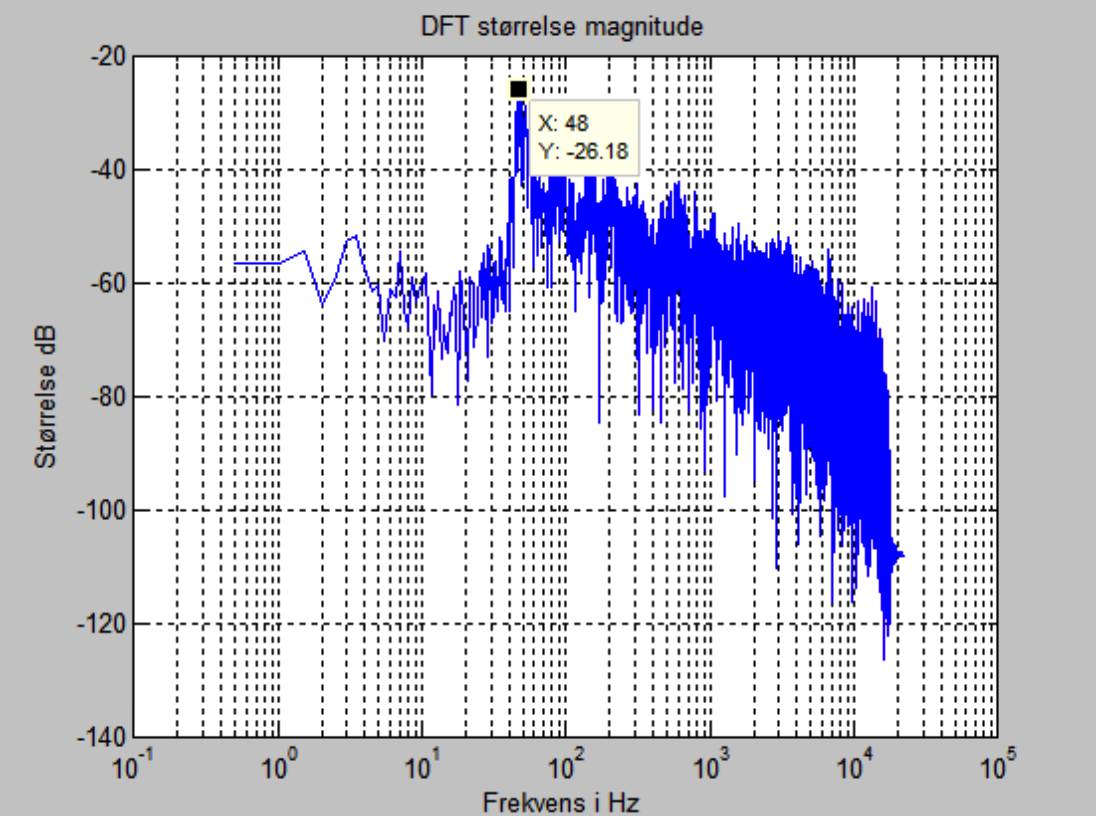
\includegraphics[width=0.7\textwidth]{Figurer/Snip20151001_18}
	\caption{\textit{Straight outta Compton} - Signalets magnitude som funktion af frekvens i Hz. Logaritmisk x-akse}
\end{figure} 

Den største amplitude har en frekvens på 48 Hz. Det er betydelig lavere end de andre musiksekvenser, der er blevet analyseret. En god forklaring på dette er, at det er en rapsang. Rap er snak - så derfor er det lavfrekvens, der er mest tydelig i denne musiksekvens.  

\begin{figure}[H]
	\centering
	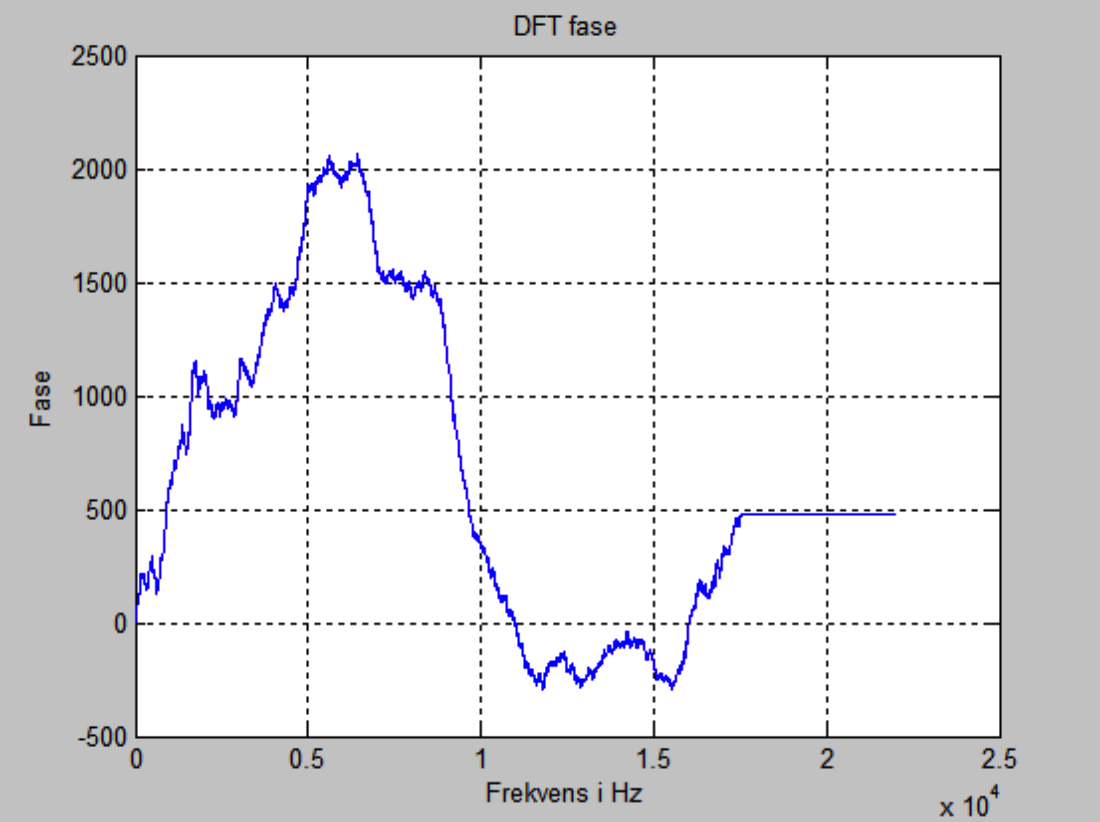
\includegraphics[width=0.7\textwidth]{Figurer/Snip20151001_19}
	\caption{\textit{Straight outta Compton} - Signalets fase som funktion af frekvens i Hz}
\end{figure} 

\section{Uptown funk}

\begin{figure}[H]
	\centering
	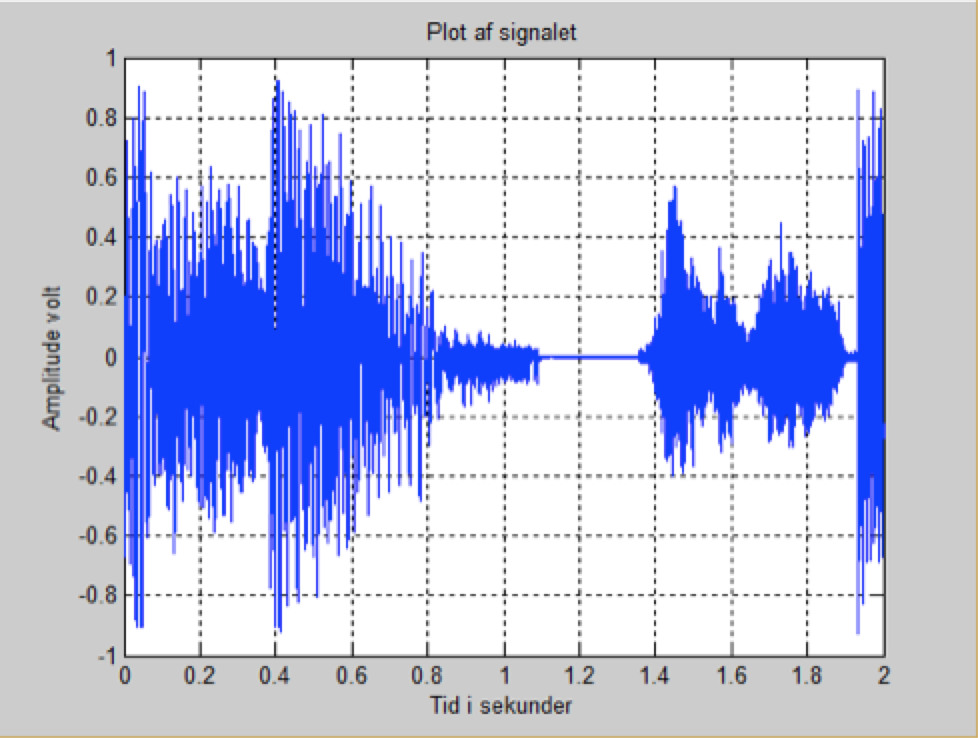
\includegraphics[width=0.7\textwidth]{Figurer/UptownFunk}
	\caption{\textit{Uptown Funk} - Signalet amplitude som funktion af tiden i sekunder}
\end{figure}

Her har vi arbejdet med sangen ”Uptown Funk”. Vi har mere specifikt kigget på en sekvens, som varer 2 sekunder midt inde i sangen. Det ses at sekvensen benytter hele amplitudespektret, og der er stor variation i amplituderne. Sekvensen er opbygget på den måde, at ca. det førte sekund oplever vi en stor opbygning, hvor musikken går helt amok og amplituderne er meget høje, indtil omkring 1.1 sekunder, hvor der kommer et break. I breaket er amplituden meget lav indtil vi kommer til 1.4 sekunder. Her sker der et anslag, og musikken starter med en opbygning igen. 

\begin{figure}[H]
	\centering
	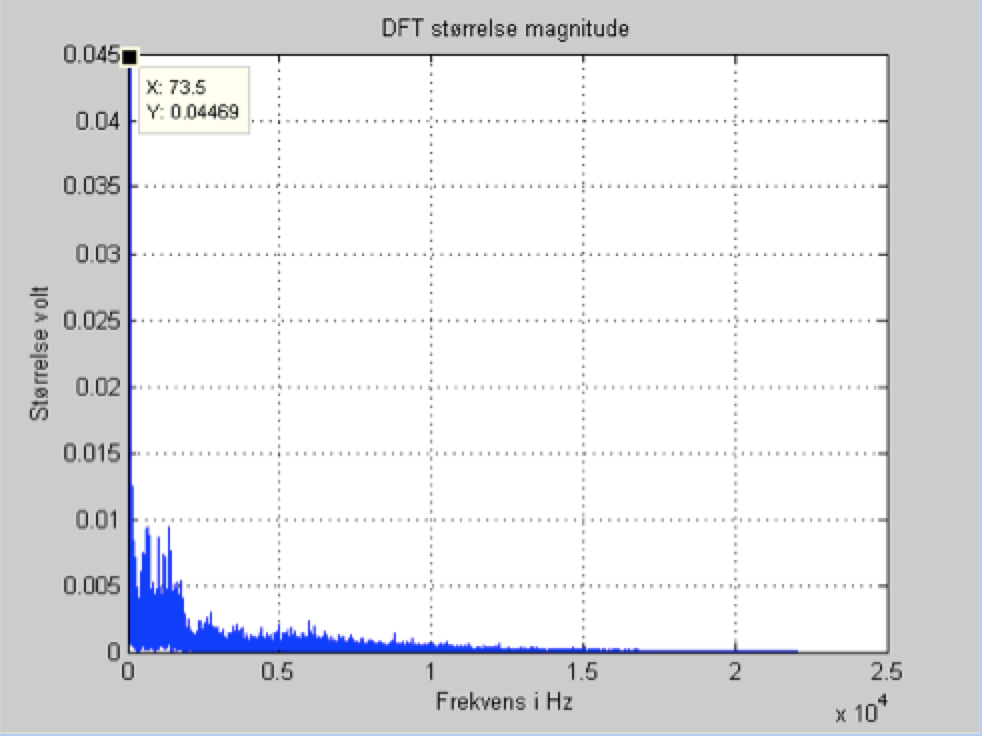
\includegraphics[width=0.7\textwidth]{Figurer/UptownFunk2}
	\caption{\textit{Uptown Funk} - Signalets magnitude som funktion af frekvens i Hz}
\end{figure}

Vi har plottet størrelsen i volt som funktion af frekvensen efter vi har fourie transformeret signalet. Her ses det at den højeste amplitude findes ved frekvensen 73.5 Hz. I den første del af sekvensen (0-500Hz), ses det at energien er meget højere end i resten af signalet. Det er typisk lave frekvenser, hvilket vil sige at de dybe toner er de mest tydelige i sangen, hvilket stemmer overens med at der er en tydelig bas i sangen.  

\begin{figure}[H]
	\centering
	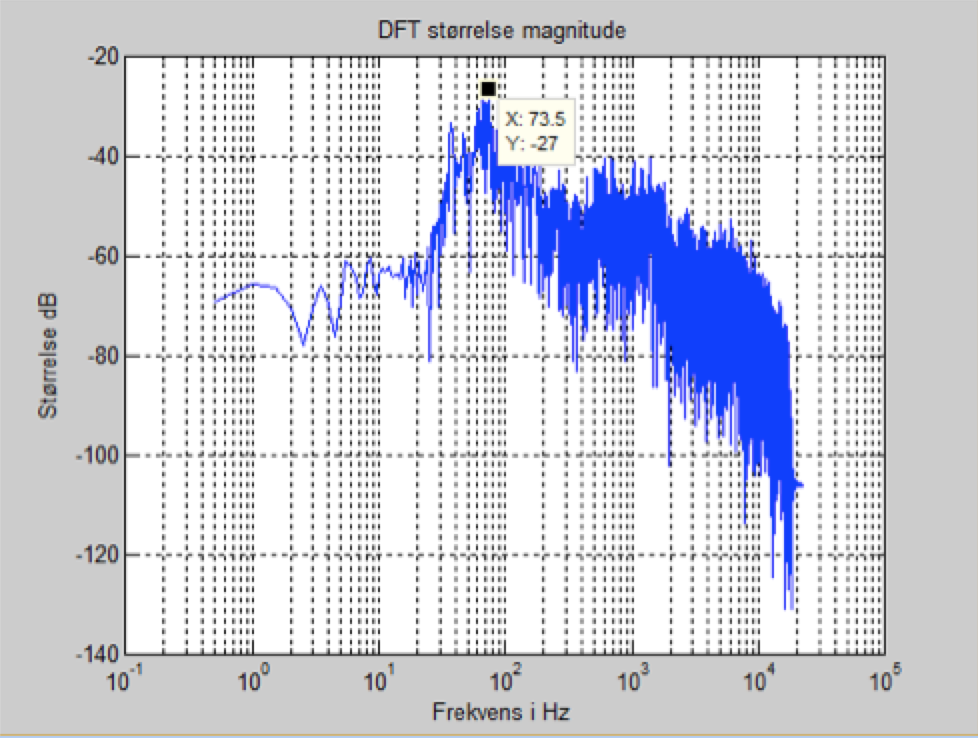
\includegraphics[width=0.7\textwidth]{Figurer/UptownFunk3}
	\caption{\textit{Uptown Funk} - Signalets magnitude som funktion af frekvens i Hz. Logaritmisk x-akse}
\end{figure}

Her er musiksekvensen plottet i størrelse i dB som funktion af frekvensen. Her er det angivet på en logaritmisk akse, for bedre at få et mere nøjagtig indblik i hvordan musiksekvensen opfører sig. Det ses at frekvensen, som har den højeste størrelse i dB stemmer overens med det forrige plot – 73.5 Hz. Det ses ligeledes her at størrelsen er størst i dB ved de lave frekvenser.

\begin{figure}[H]
	\centering
	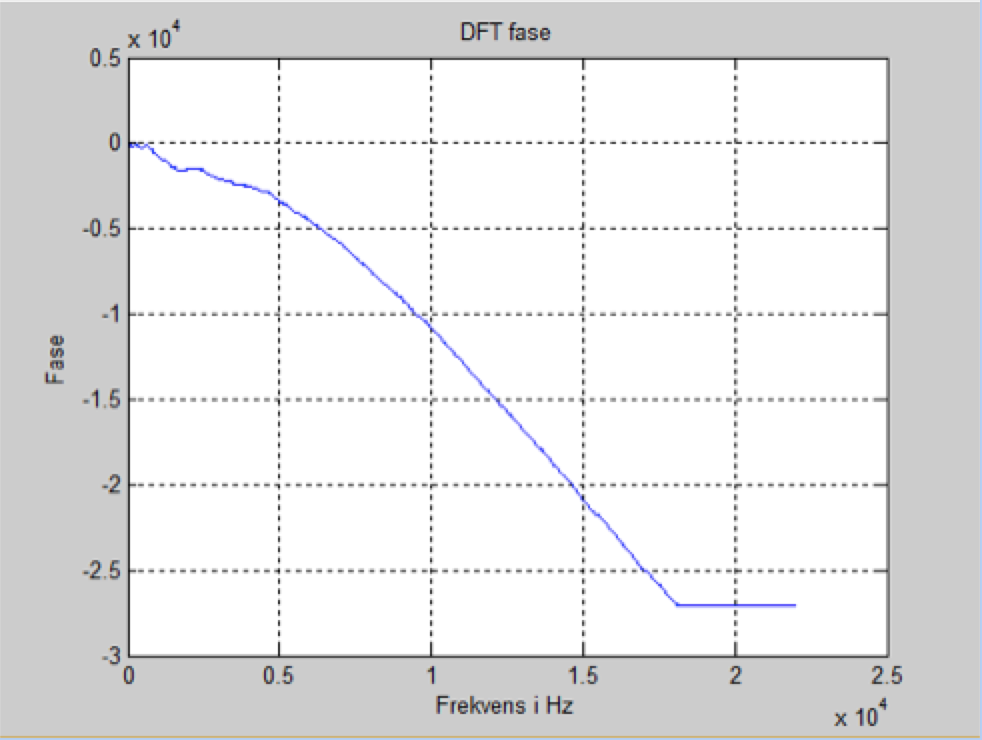
\includegraphics[width=0.7\textwidth]{Figurer/UptownFunk4}
	\caption{\textit{Uptown Funk} - Signalets fase som funktion af frekvens i Hz}
\end{figure}

Her er fasen plottet som funktion af frekvensen. Det ses at fasen falder kontinuerligt fra ca. 0-18000 Hz.

\section{Der er et yndigt land}

\begin{figure}[H]
	\centering
	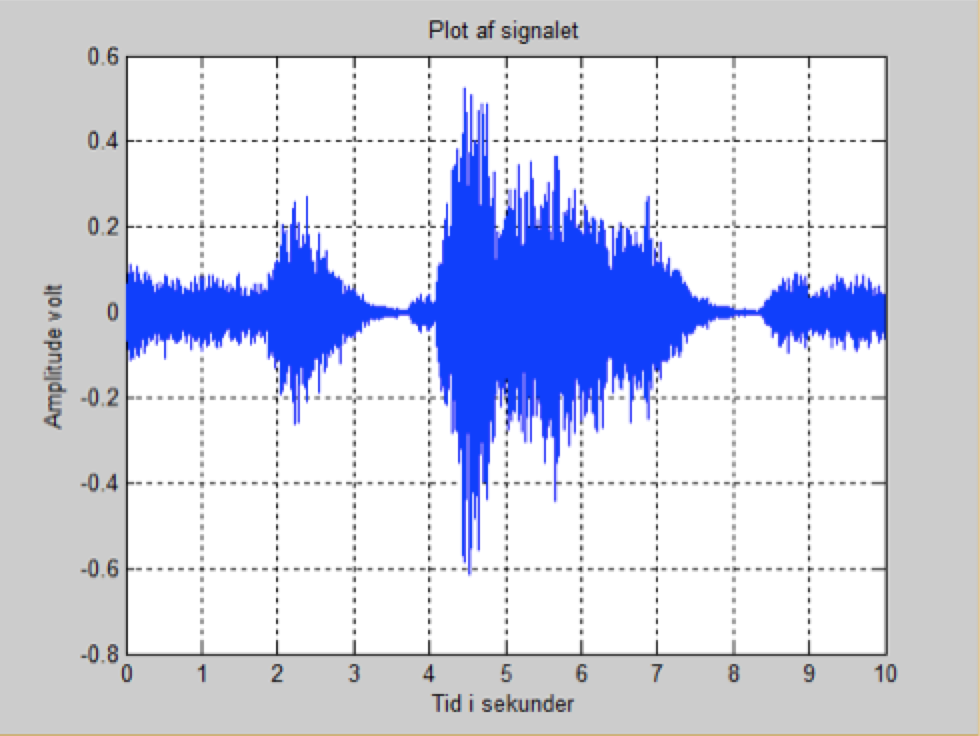
\includegraphics[width=0.7\textwidth]{Figurer/Nationalsang}
	\caption{\textit{Der er et yndigt land} - Signalet amplitude som funktion af tiden i sekunder}
\end{figure}

Her har vi arbejdet med en stykke klassisk musik med sang ind over. Nærmere betegnet vores nationalmelodi – ”Der er et yndigt land”. Klippet varer 10 sekunder, og det ses at amplitudespektret er meget varierende i hele musiksekvensen. Det ses bl.a. ved omkring 3-5 sekunder, hvor musikken bliver helt stille, og derefter kommer der et kæmpe anslag med en høj amplitude.

\begin{figure}[H]
	\centering
	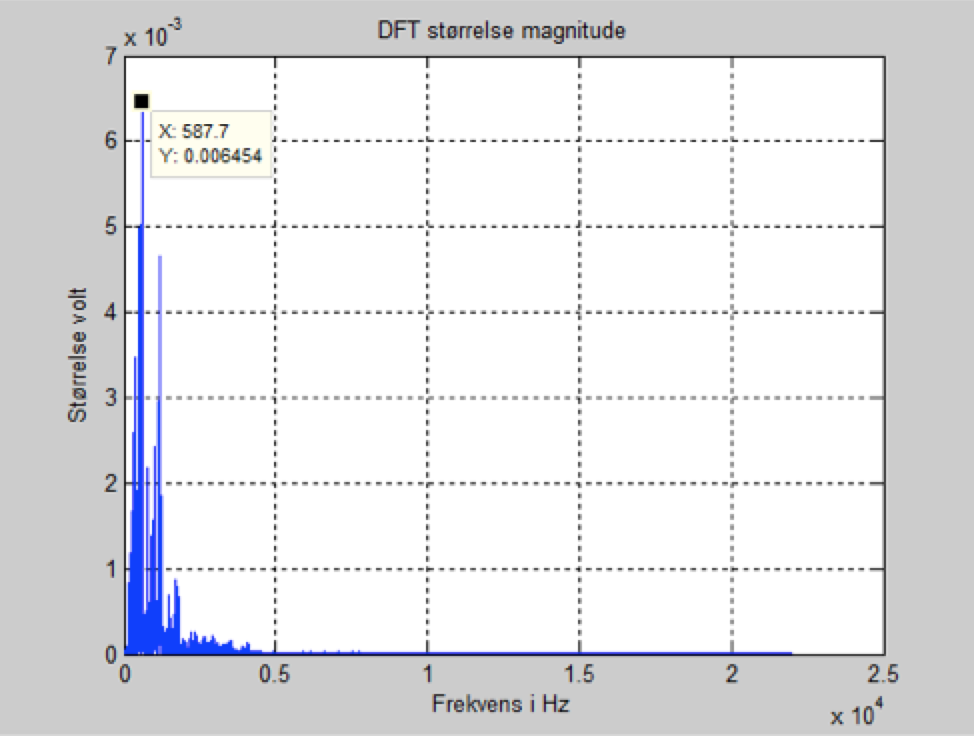
\includegraphics[width=0.7\textwidth]{Figurer/Nationalsang2}
	\caption{\textit{Der er et yndigt land} - Signalets magnitude som funktion af frekvens i Hz}
\end{figure}

Efter vi har fourie tranformeret vores signal, har vi plottet størrelsen i volt som funktion af frekvensen. Her ses det at den højeste amplitude findes ved frekvensen 587.7 Hz. I den første del af sekvensen (0-1200 Hz), ses det at energien er meget højere end i resten af signalet. 

\begin{figure}[H]
	\centering
	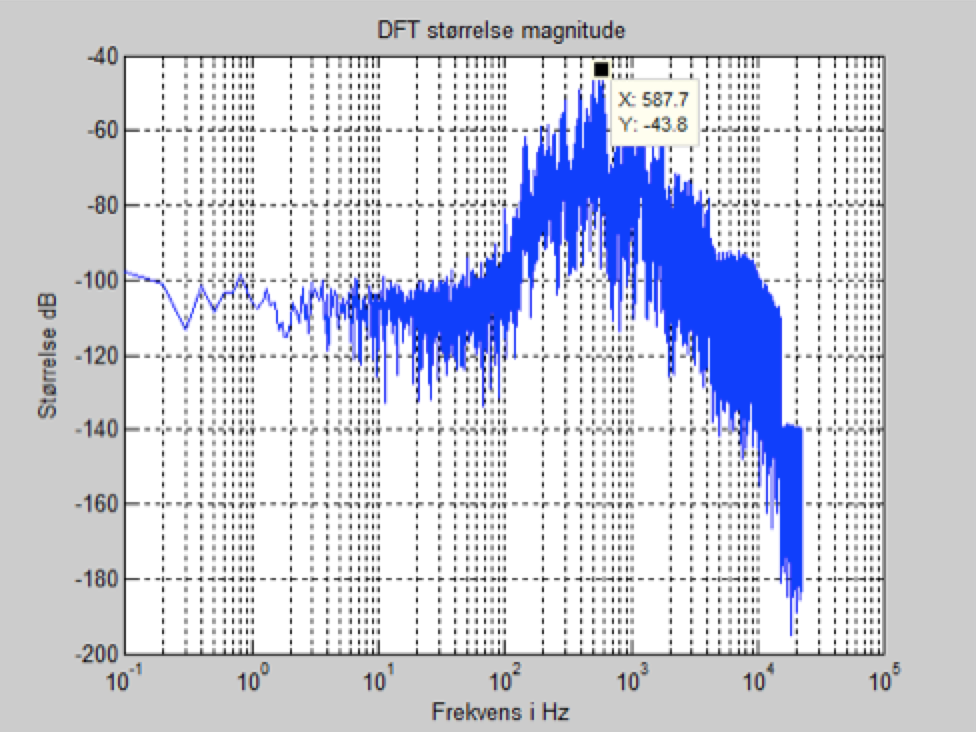
\includegraphics[width=0.7\textwidth]{Figurer/Nationalsang3}
	\caption{\textit{Der er et yndigt land} - Signalets magnitude som funktion af frekvens i Hz. Logaritmisk x-akse}
\end{figure}

Her er signalet plottet ved størrelsen i dB som funktion af frekvensen i Hz i en logaritmisk skala. Dette gøres for bedre at kunne analysere på signalet. Det ses at den største størrelse dB er ved 587.7 Hz, hvilket passer med det foregående plot. 587.7 Hz er faktisk lige præcis tonen D5. 

\begin{figure}[H]
	\centering
	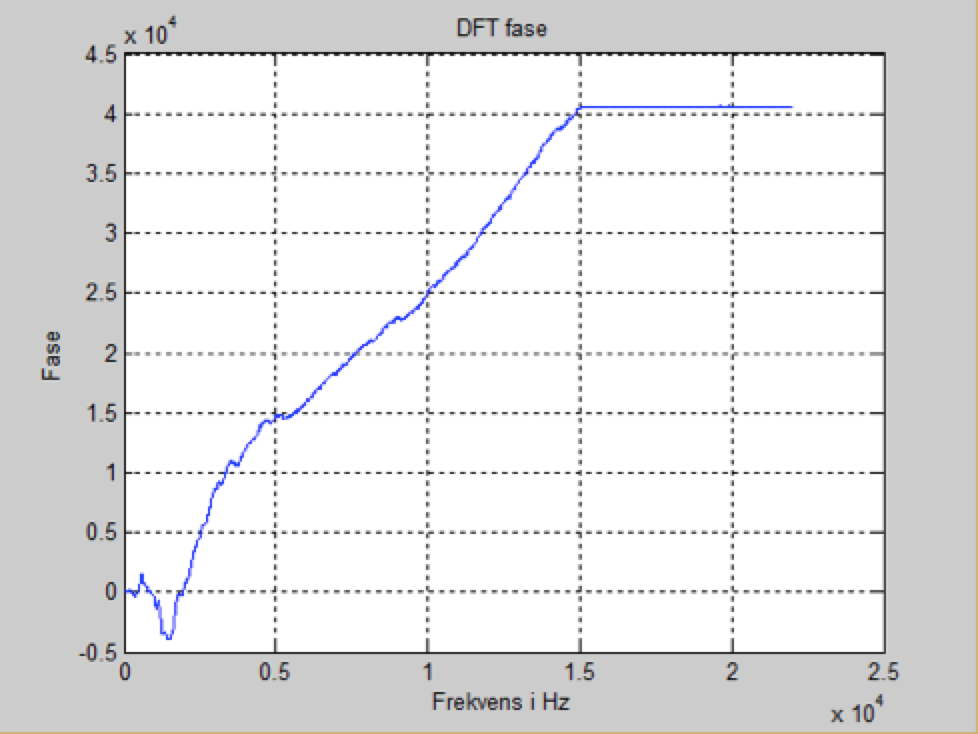
\includegraphics[width=0.7\textwidth]{Figurer/Nationalsang4}
	\caption{\textit{Der er et yndigt land} - Signalets fase som funktion af frekvens i Hz}
\end{figure}

Her er fasen plottet som funktion af frekvensen. Der sker en fasedrejning ved ca. 1400 Hz. Herefter ses det at fasen stiger kontinuerligt indtil omkring 15000 Hz, hvorefter den forbliver konstant.


\chapter{EKG}
I dette afsnit vil der blive analyseret et fysiologisk signal, som vi har hentet ned fra PhysioNet. Mere præcist, vil der blive analyseret et EKG signal. \\
Der vil være 4 forskellige grafer for E.\\ \\
Den først viser signalet som funktion af tiden - her befinder signalet sig i tidsdomænet. \\
De 2 næste viser signalet magnitude som funktion af frekvens i Hz. Den sidste af disse viser signalet på en logaritmisk x-akse. \\
Den sidste graf viser fasen som funktion af frekvens i Hz. De sidste 3 befinder sig frekvens-domænet, da vi har lavet en DFT af signalet.


\section{EKG}

\begin{figure}[H]
	\centering
	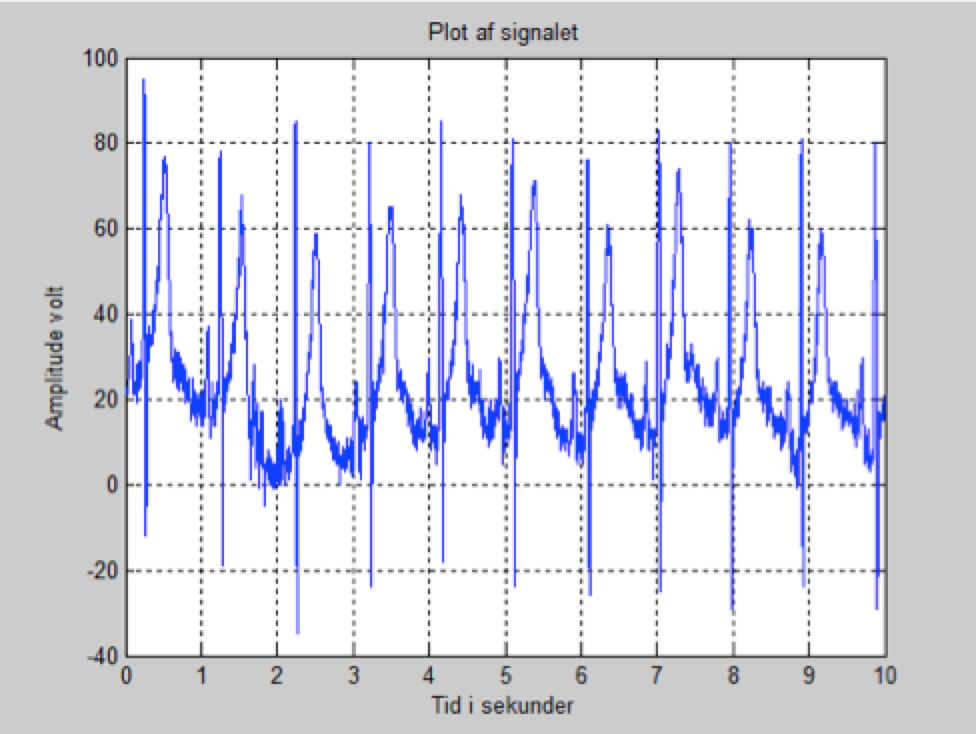
\includegraphics[width=0.7\textwidth]{Figurer/EKG}
	\caption{\textit{EKG} - Signalet amplitude som funktion af tiden i sekunder}
\end{figure}

Dette er et EKG-signal som er et noget anderledes signal sammenlignet med de tidligere musikeksempler. Signalet er på 10 sekunder, og det er afbilledet ved amplituden i volt som funktion af tiden i sekunder. Et EKG-signal har store svingninger i amplituden, alt efter om vi fx er ved r-takkerne, q-takkerne eller nogle af de andre takker. Når hjertet slår og trækker sig sammen, får vi nogle impulser, som bliver omdannet til elektriske signaler hvilket er afbilledet på EKG-signaler. De høje amplituder kommer hver gang, der er et pulslag. Det ses at vi arbejder med nogle meget højere amplituder i volt end i de foregående musikeksempler. 

\begin{figure}[H]
	\centering
	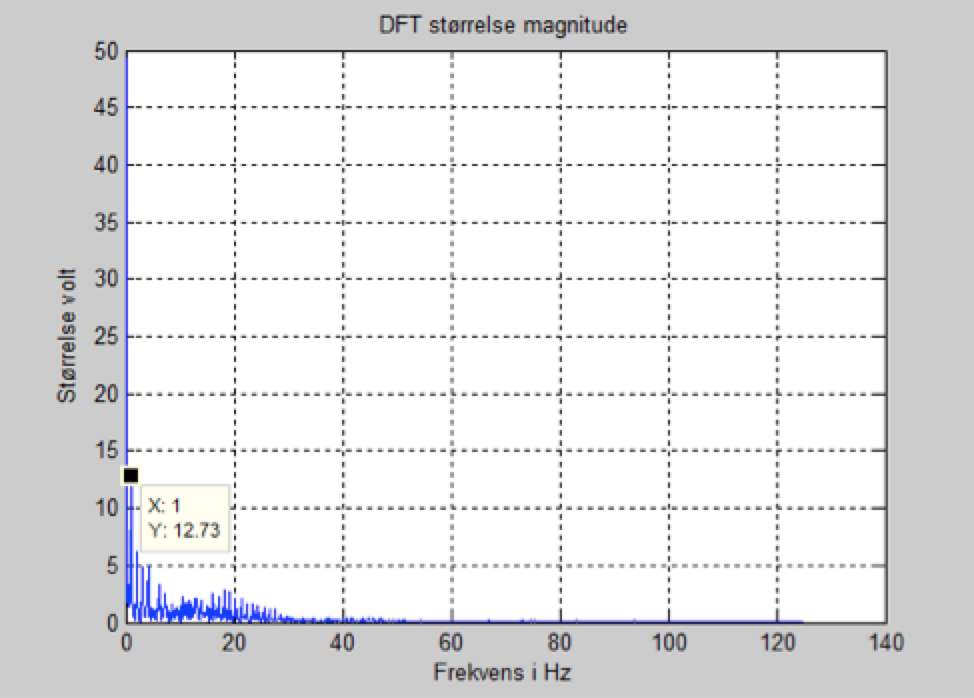
\includegraphics[width=0.7\textwidth]{Figurer/EKG2}
	\caption{\textit{EKG} - Signalets magnitude som funktion af frekvens i Hz}
\end{figure}

Her har vi fourie tranformeret signalet, og plottet det ved størrelsen i volt som funktion af frekvensen i Hz. Det er hurtigt i øjenfaldende, at vi arbejder med nogle meget lavere frekvenser, end ved musikeksemplerne. Den største energi i signalet ligger ca. ved frekvenserne 0-6 Hz. Mens den har et højdepunkt ved 1 Hz. Det ses også at størrelserne bliver mindre jo højere frekvens, og at den er hurtigt faldende ved de 20 Hz. 

\begin{figure}[H]
	\centering
	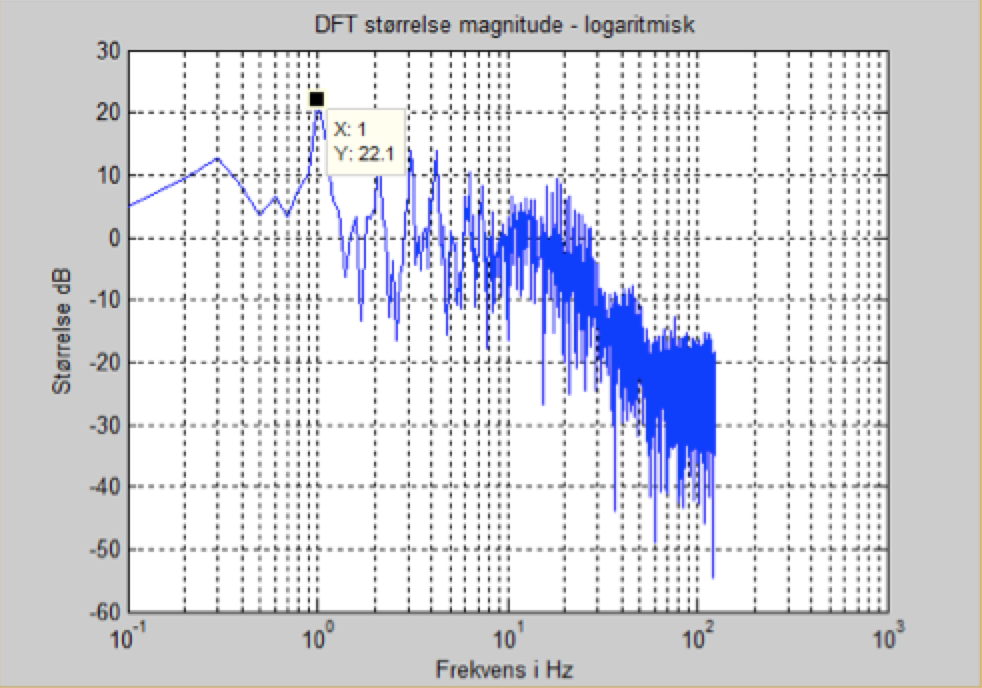
\includegraphics[width=0.7\textwidth]{Figurer/EKG3}
	\caption{\textit{EKG} - Signalets magnitude som funktion af frekvens i Hz. Logaritmisk x-akse}
\end{figure}

Her er signalet plottet ved størrelsen i dB som funktion af frekvensen i Hz i en logaritmisk skala. Dette gøres for bedre at kunne analysere på signalet. Det ses at der er store udsving i størrelserne for de forskellige frekvenser, indtil omkring 10 Hz, hvor det begynder at blive mere tæt. Der er et toppunkt ved frekvensen 1 Hz, hvilket stemmer overens med det tidligere plot. Der er mest energi i signalet fra ca. 0-7 Hz.

\begin{figure}[H]
	\centering
	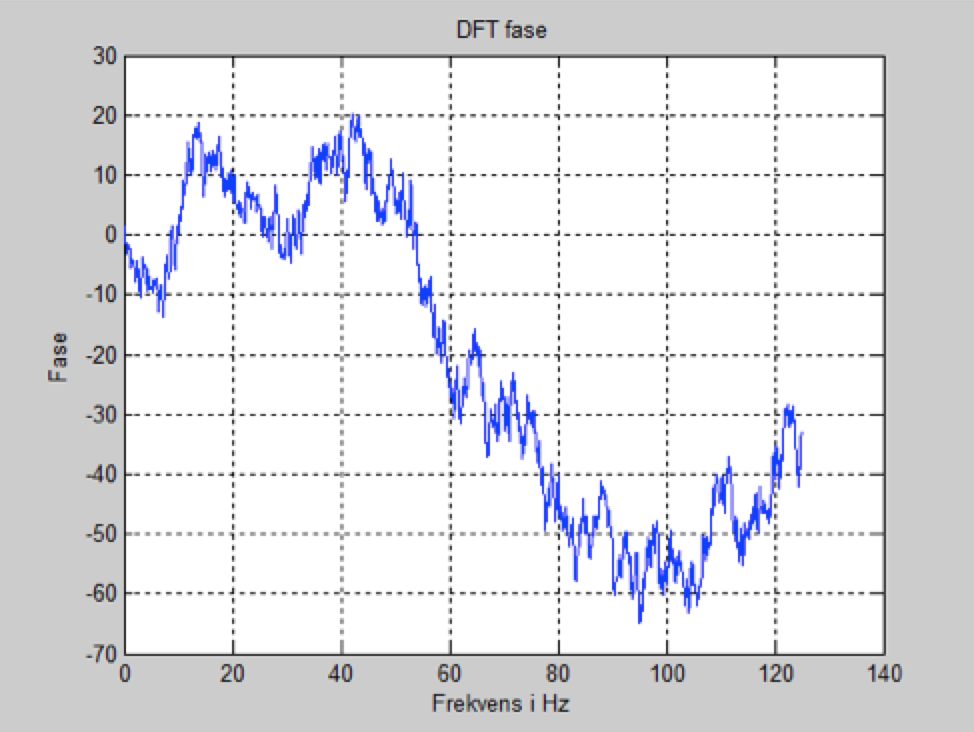
\includegraphics[width=0.7\textwidth]{Figurer/EKG4}
	\caption{\textit{EKG} - Signalets fase som funktion af frekvens i Hz}
\end{figure}

Her er det fourie transformeret signals fase afbilledet som funktion af frekvensen i Hz. Fasen for EKG-signalet er meget forskelligt fra musiksekvensere. Musiksekvensernes fase var mere varierende, sammenlignet med fasen for EKG-signalet. Der foregår fasedrejninger hele tiden, og den kører op og ned. Generelt kan man sige at fasen stiger og falder i starten indtil de 40 Hz. Herefter falder fasen til vi når til 100 Hz, hvorefter den stiger igen. 


\chapter{Vind}
I dette afsnit vil der blive analyseret et signal fra en vindmølle. \\
Der vil være 4 forskellige grafer for signalet.\\ \\
Den først viser signalet som funktion af tiden - her befinder signalet sig i tidsdomænet. \\
De 2 næste viser signalet magnitude som funktion af frekvens i Hz. Den sidste af disse viser signalet på en logaritmisk x-akse. \\
Den sidste graf viser fasen som funktion af frekvens i Hz. De sidste 3 befinder sig frekvens-domænet, da vi har lavet en DFT af signalet.


\section{Vind}

\begin{figure}[H]
	\centering
	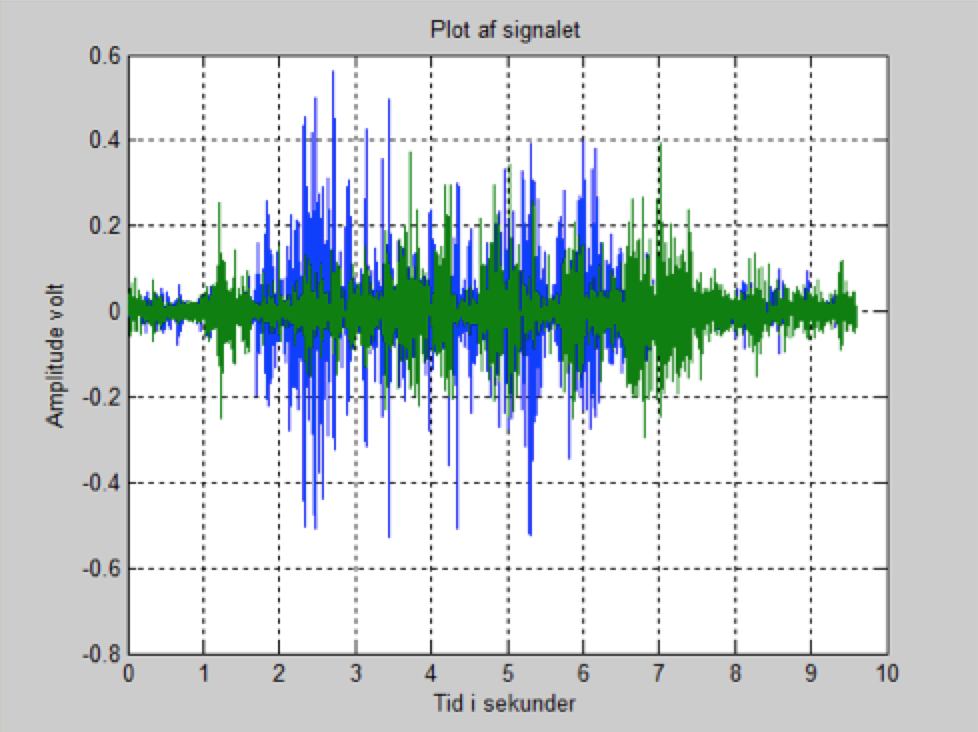
\includegraphics[width=0.7\textwidth]{Figurer/Vind}
	\caption{\textit{Vind} - Signalet amplitude som funktion af tiden i sekunder}
\end{figure}

Det først man kan ligge mærke til, er at der både er en blå og en grøn graf. Der er altså 2 kanaler. Ene er muligvis en udtryk for vinden og den anden for selve vindmøllen. Når man lytter til lydsekvensen kan man ca. 2 sekunder inde hører vinden kraftigt - derfor vil vi mene, at den blå er for vinden, da den har det største amplituder. Den grønne, som så er for selve vindmøllen, er mere centraliseret omkring 0 - altså, der er ikke så store udsving i amplituden.  

\begin{figure}[H]
	\centering
	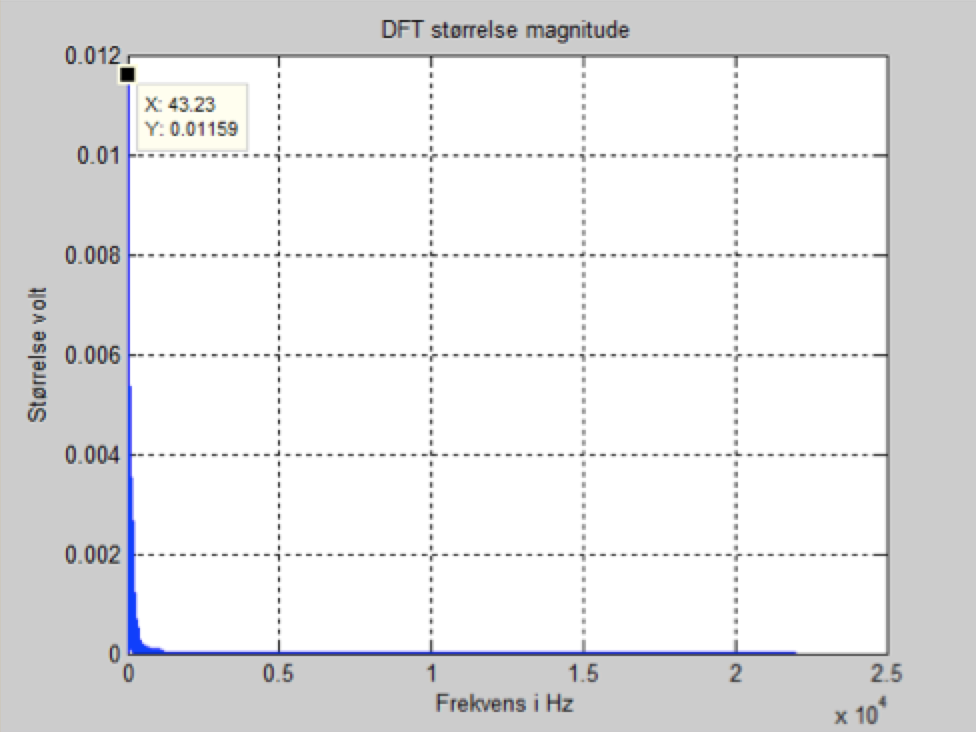
\includegraphics[width=0.7\textwidth]{Figurer/Vind2}
	\caption{\textit{Vind} - Signalets magnitude som funktion af frekvens i Hz}
\end{figure}

Den størte amplitude ligger ved 43,23 Hz. Det er i den lave ende, hvilket stemmer overens med, at det er en meget brummende lyd, sådan en vindmølle kan lave. Lydsekvensen er derfor præget af lavfrekvens. 

\begin{figure}[H]
	\centering
	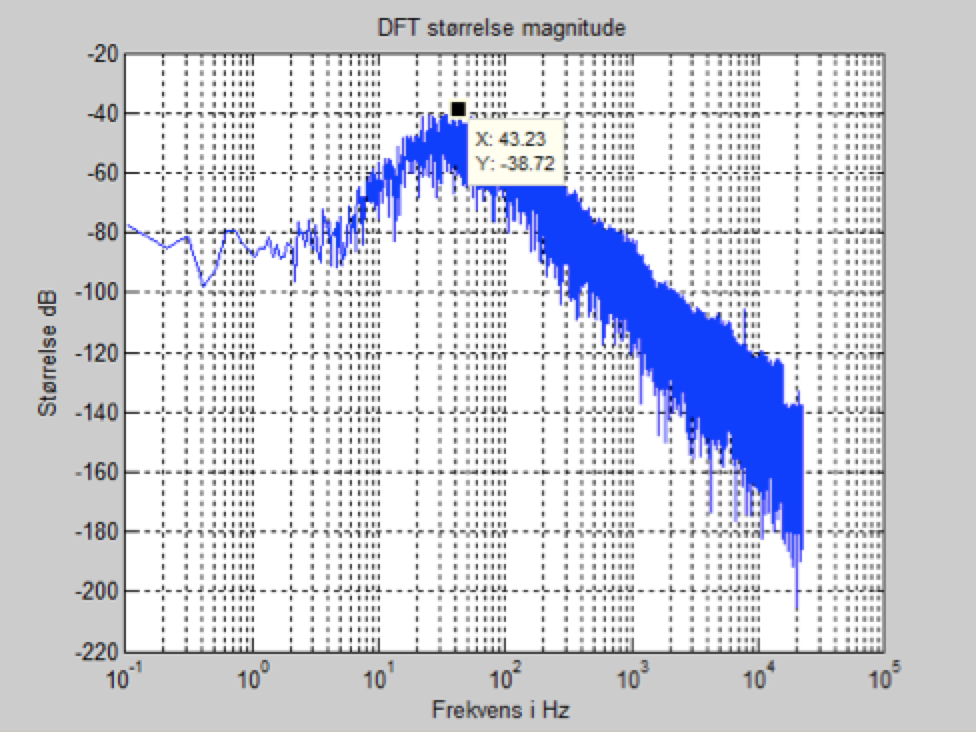
\includegraphics[width=0.7\textwidth]{Figurer/Vind3}
	\caption{\textit{Vind} - Signalets magnitude som funktion af frekvens i Hz. Logaritmisk x-akse}
\end{figure}

Her er signalet plottet ved størrelsen i dB som funktion af frekvensen i Hz i en logaritmisk skala. Dette gøres for bedre at kunne analysere på signalet. Den frekvens med den største energi, dB, er det samme på forrige bilde - hvilket der også forventes. 

\begin{figure}[H]
	\centering
	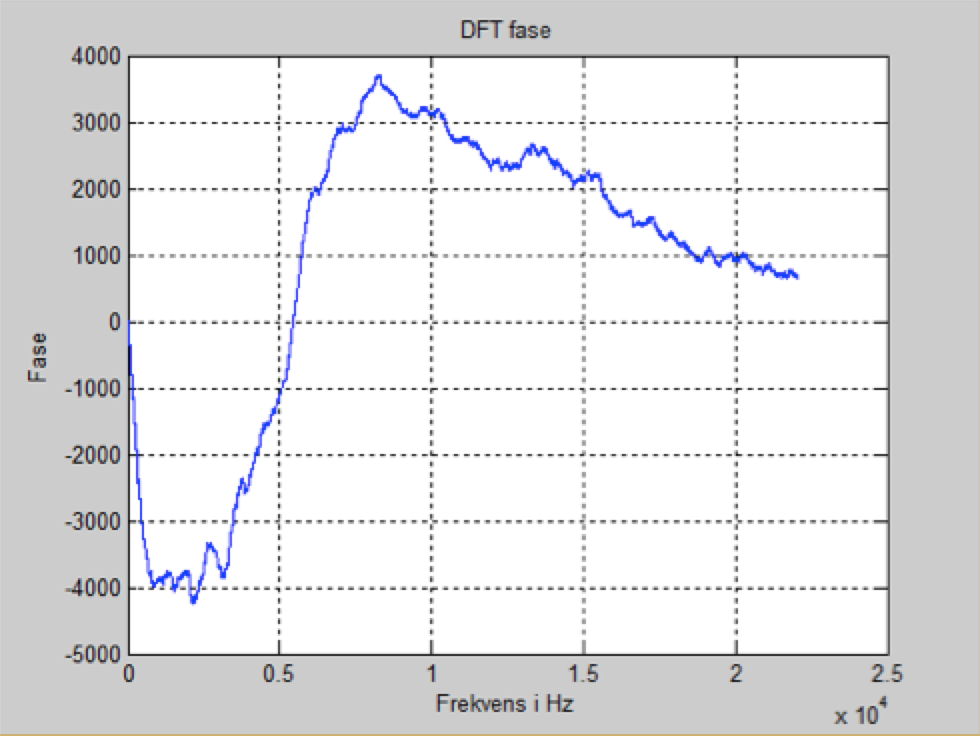
\includegraphics[width=0.7\textwidth]{Figurer/Vind4}
	\caption{\textit{Vind} - Signalets fase som funktion af frekvens i Hz}
\end{figure}

Hvis vi kigger på fasekarakteristikken for signalet fra vindmøllen, kan vi se der sker nogle fasedrejninger i mellem intervallet 0-500 Hz, hvorefter den forbliver nogenlunde stabil til omkring 800 Hz. Herefter forekommer der igen en masse små fasedrejninger dog primært i negativ retning.  


\chapter{Bil}
I dette afsnit vil der blive analyseret et signal fra en bil. \\
Der vil være 4 forskellige grafer for signalet.\\ \\
Den først viser signalet som funktion af tiden - her befinder signalet sig i tidsdomænet. \\
De 2 næste viser signalet magnitude som funktion af frekvens i Hz. Den sidste af disse viser signalet på en logaritmisk x-akse. \\
Den sidste graf viser fasen som funktion af frekvens i Hz. De sidste 3 befinder sig frekvens-domænet, da vi har lavet en DFT af signalet.


\section{Bil}

\begin{figure}[H]
	\centering
	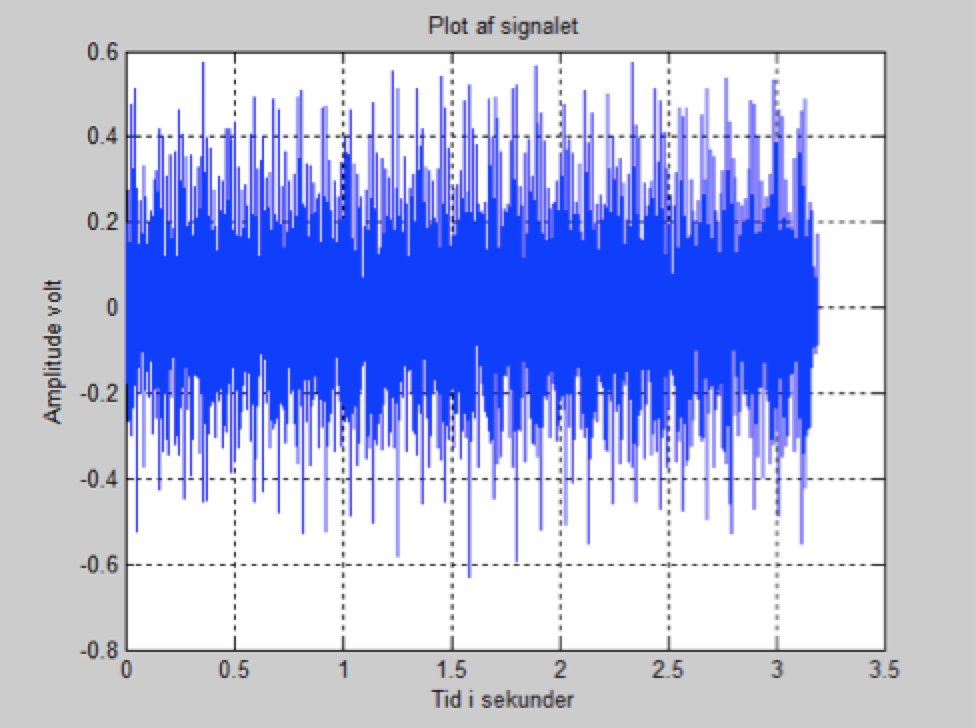
\includegraphics[width=0.7\textwidth]{Figurer/Bil}
	\caption{\textit{Bil} - Signalet amplitude som funktion af tiden i sekunder}
\end{figure}

Det ses at signalet forholder sig forholdsvis monotont og der sker ikke nogle markante udsving, som vi fx så i de fleste musiksekvenser. 

\begin{figure}[H]
	\centering
	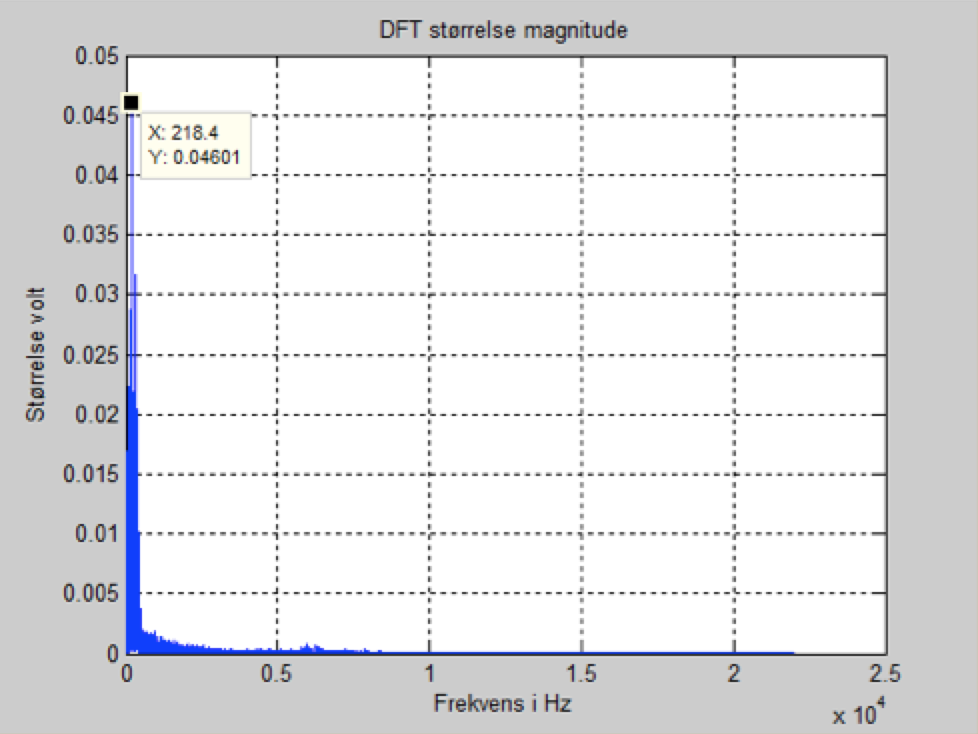
\includegraphics[width=0.7\textwidth]{Figurer/Bil2}
	\caption{\textit{Bil} - Signalets magnitude som funktion af frekvens i Hz}
\end{figure}

Signalets energi er igen størst ved de lavere frekvenser, ligesom det har været med de fleste andre signaler vi har analyseret. Her er sker faldet dog ved en lidt lavere frekvens end tidligere. Allerede ved ca. 1000 Hz er volt omkring 0.

\begin{figure}[H]
	\centering
	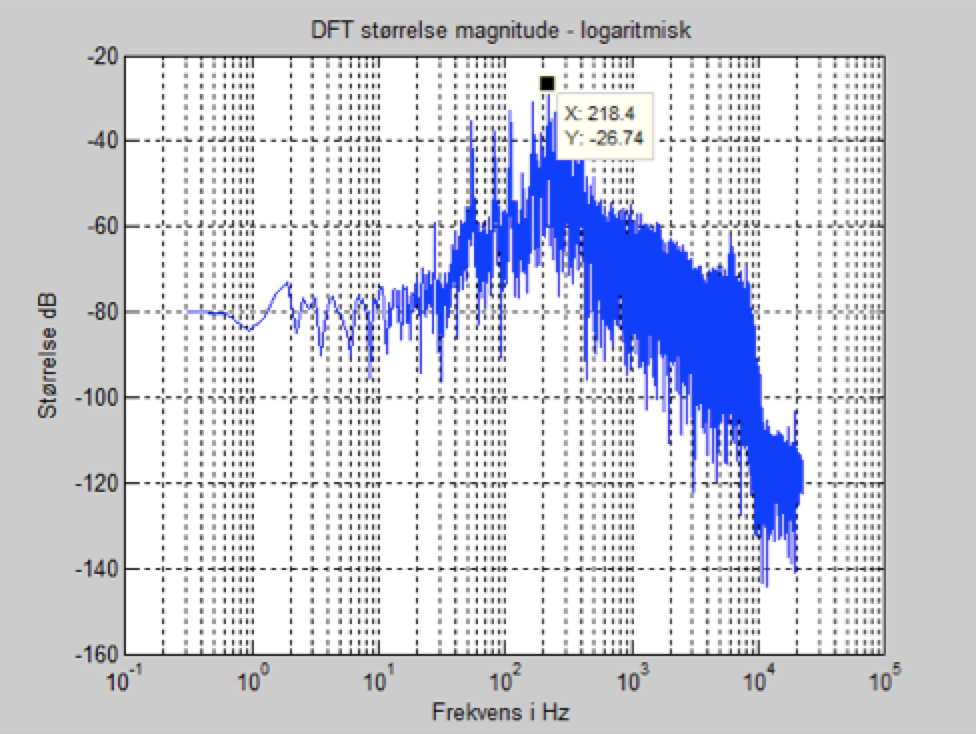
\includegraphics[width=0.7\textwidth]{Figurer/Bil3}
	\caption{\textit{Bil} - Signalets magnitude som funktion af frekvens i Hz. Logaritmisk x-akse}
\end{figure}

Hvis vi kigger på størrelsen i dB, så er det interessant at kigge på frekvenserne fra omkring 30 Hz og frem til 500 Hz, da frekvensernes størrelse i dB i dette interval er en del større, end de resterende frekvenser. Desuden ligger punkterne en del tættere fra omkring 200 Hz og fremefter ift. til de mindre frekvenser.

\begin{figure}[H]
	\centering
	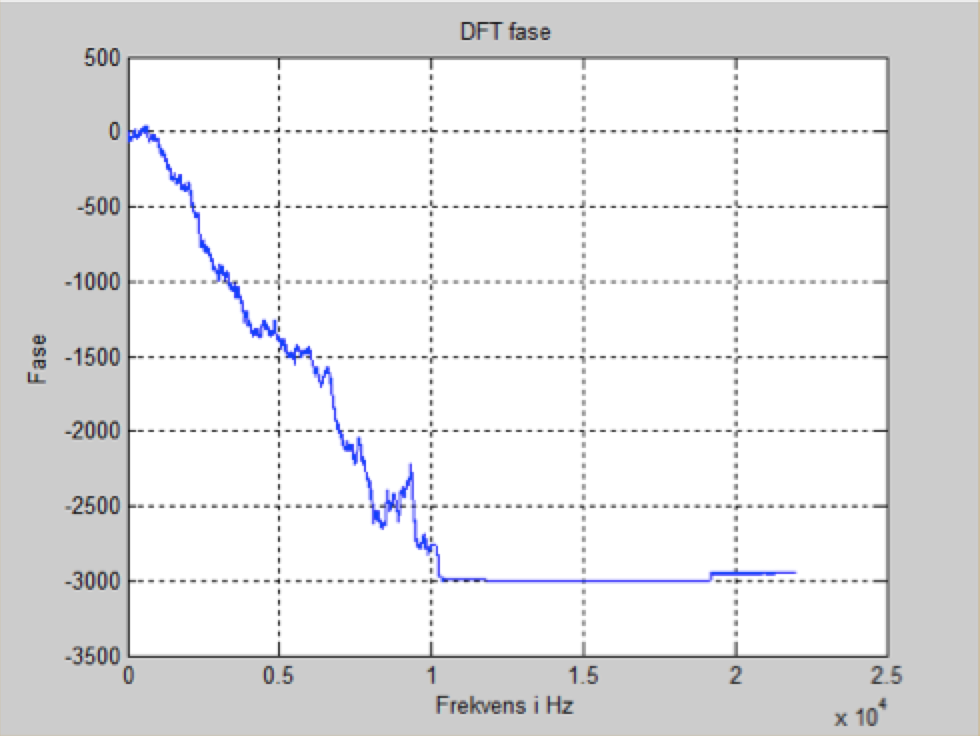
\includegraphics[width=0.7\textwidth]{Figurer/Bil4}
	\caption{\textit{Bil} - Signalets fase som funktion af frekvens i Hz}
\end{figure}

Hvis vi kigger på fasekarakteristikken for signalet fra bilen, ses det at der sker et kontinuerligt fra omkring 300 Hz og ned til 10000 Hz, hvorefter det forholder sig lineært ad x-aksen.









